%------------------------------------------------------------------------------
% Method
%------------------------------------------------------------------------------

\section{Method}
\label{sec:method}

Given a single oil painting $I_p \in \mathbb{R}^{H\times W\times 3}$,
Paint2World produces a 3D-consistent flythrough video
$\{I_t\}_{t=1}^{N}$ and a 3D Gaussian Splatting scene $\mathcal{G}$ that
reproduces the painting from its viewpoint and can be rendered from novel
views. The pipeline has five stages (Fig.~\ref{fig:method}): Stage -1
(painting analysis), Stage -0.5 (object-level scene construction: object
segmentation, TripoSplat-style 3D object generation, spatial-dependency
graph, scene canvas), Stage 0 (canvas-conditioned video generation), Stage 1
(painting-anchored non-rigid alignment), and Stage 3.2 (stroke-coherent,
object-rigid 3GS).

\subsection{Design rationale: why the painting is a 3D-stability prior}
\label{sec:design}

A natural question is why a 2D painting should help 3D consistency at all.
We identify four properties of human oil paintings that make them
particularly suitable canonical priors, and each motivates one of our
stability mechanisms.

\paragraph{(D1) Deliberate depth composition.}
Unlike a photograph, an oil painting encodes an artist-chosen depth layout:
the horizon placement, the chiaroscuro, and the foreground/background
separation are all compositional decisions. This makes the painting's
estimated depth $D_p$ a \emph{layout prior} that is more reliable than any
single generated frame's depth. This motivates the \emph{depth-warp geometry
control} (Stage 0, \S\ref{sec:stage0}) and the \emph{painting-anchored
canonical initialisation} (Stage 1, \S\ref{sec:stage1}): we pin every
generated frame's geometry and the canonical frame itself to $D_p$.

\paragraph{(D2) Explicit brush-stroke structure.}
Oil paintings are composed of discrete brush strokes, each a coherent surface
patch with relatively uniform colour. This stroke structure is a strong
\emph{correspondence prior}: a stroke visible in the painting should remain a
single coherent 3D patch across all generated views. This motivates the
\emph{stroke-consistency temporal-attention bias} (Stage 0) and the
\emph{stroke-coherence GS loss} (Stage 3.2, \S\ref{sec:stage3}).

\paragraph{(D3) Authoritative appearance.}
The painting is the user's ground-truth appearance for the reference
viewpoint. Any 3D scene generated from it must reproduce the painting when
rendered from $T_1$. This motivates the \emph{painting-view reconstruction
loss} (Stage 3.2), which anchors the optimised Gaussians to the artwork and
prevents the scene from drifting toward a plausible-but-wrong appearance.

\paragraph{(D4) Compositional object structure.}
An oil painting depicts \emph{things} --- trees, vessels, faces, buildings ---
each painted as a coherent unit and arranged deliberately in depth: the
artist decides what rests on what, what occludes what, and where the ground
lies. This motivates the \emph{object-level scene canvas} (Stage -0.5,
\S\ref{sec:stage-object}): segment the painting into objects, generate each
object's 3D geometry, and compose them through an explicit
spatial-dependency graph; the canvas then supplies the geometry control for
Stage 0 and the rigid anchors + relation-preservation constraints for
Stage 3.2.

\begin{figure*}[t]
\centering
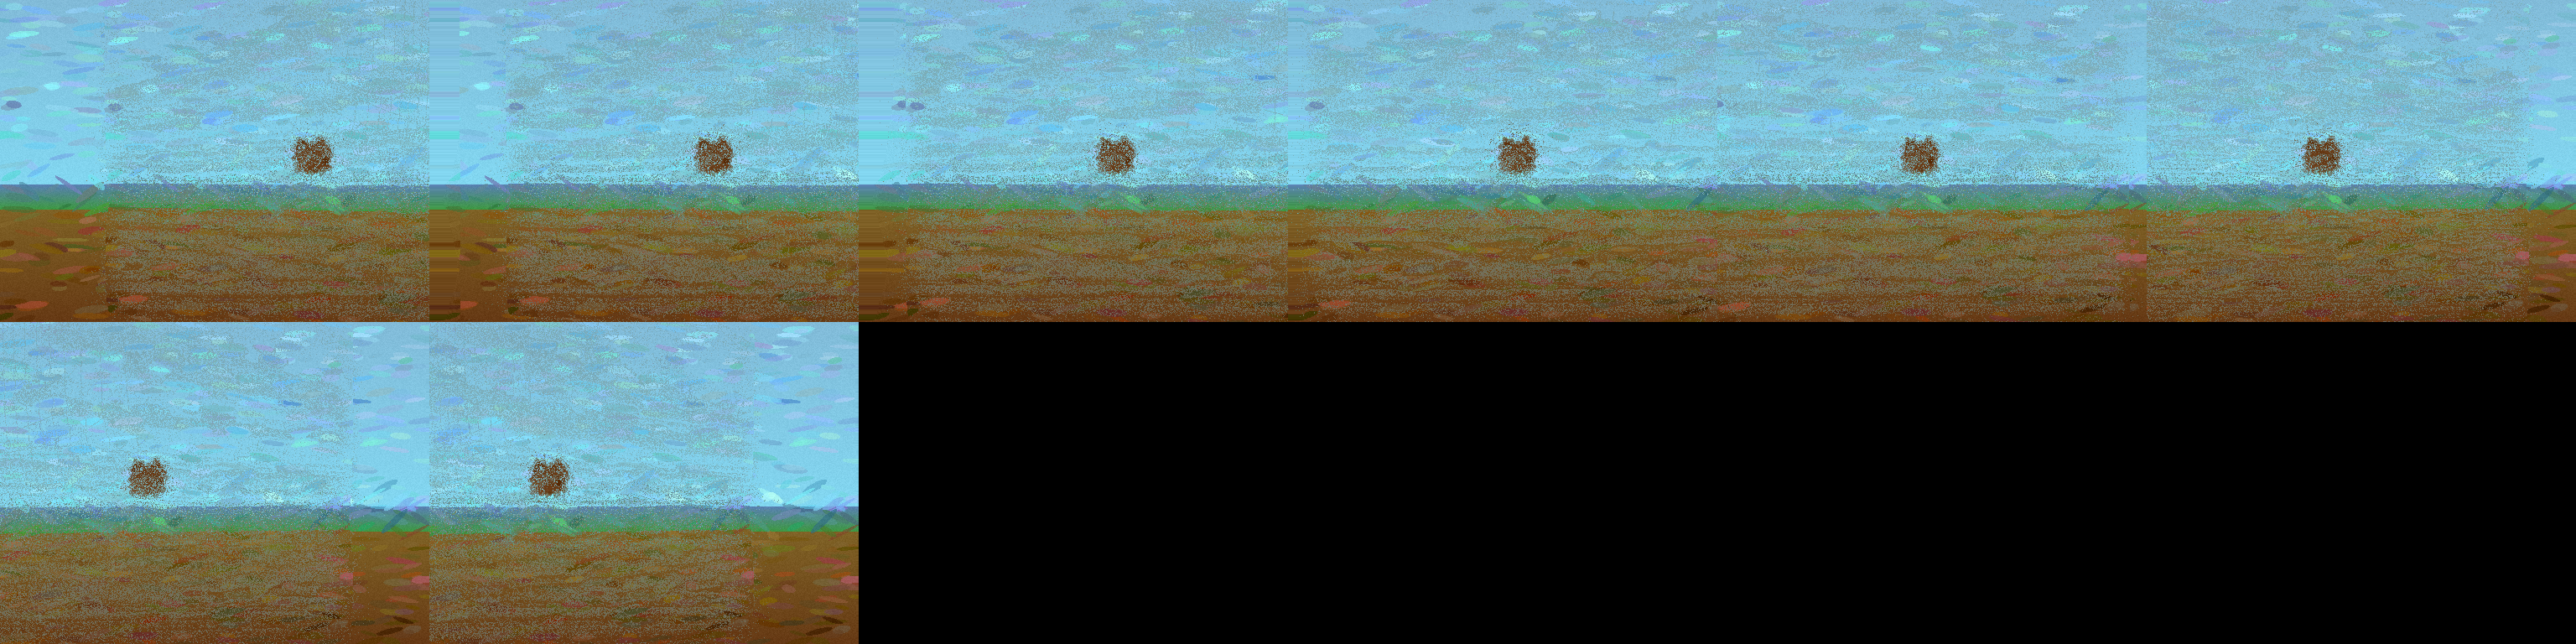
\includegraphics[width=0.95\linewidth]{figures/teaser_frames.png}
\caption{\textbf{Pipeline overview.} Stage -1 estimates depth, normals, and
brush-stroke segmentation from the painting. Stage -0.5 segments the painting
into objects, generates each object in 3D with a TripoSplat-style
triplane-to-Gaussian decoder, and composes them onto a 3D scene canvas with
an explicit spatial-dependency graph. Stage 0 generates a 3D-stable
flythrough whose per-frame geometry is constrained by a canvas-composited
depth-warp control and whose temporal attention is biased by the painting's
strokes. Stage 1 non-rigidly aligns the generated frames into a
painting-initialised canonical cloud. Stage 3.2 trains a stroke-coherent,
object-rigid 3DGS scene.}
\label{fig:method}
\end{figure*}

% ---------------------------------------------------------------------
\subsection{Stage -1: Painting analysis}
\label{sec:stage-1}

We estimate three maps from the painting: a monocular depth map $D_p$, a
surface-normal map $N_p$, and a brush-stroke segmentation $S_p \in
\mathbb{N}^{H\times W}$. In the production deployment $D_p$ is predicted by
DepthAnything-3~\cite{da3} and $S_p$ by SAM2~\cite{sam2}; in the
out-of-the-box demo we use a \emph{perceptual synthetic depth estimator} that
combines atmospheric perspective, a soft horizon prior, local contrast, and
relative luminance cues into a depth map in $[0,1]$, and an oriented-gradient
superpixel grouping for strokes. We also compute a confidence map $C_p$ that
is high in textured stroke regions and low in flat sky/ground. The depth and
confidence are unprojected into a coloured point cloud
$\mathcal{P}_p = \{(x_i, c_i, n_i, w_i)\}$ that serves as the canonical-frame
prior.

% ---------------------------------------------------------------------
\subsection{Stage -0.5: Object-level scene construction}
\label{sec:stage-object}

The stroke map $S_p$ models the painting's \emph{marks}; the canvas stage
models its \emph{things}. It produces an explicit 3D scene scaffold
$\mathcal{C}$ --- the \emph{scene canvas} --- in three steps
(Fig.~\ref{fig:canvas}).

\paragraph{Depth-aware object segmentation.}
We segment the painting into object instances $M_o \in
\mathbb{N}^{H\times W}$. In production $M_o$ comes from SAM2 /
Mask2Former~\cite{sam2,mask2former}; the demo uses a synthetic backend that
clusters pixels jointly in LAB colour and estimated-depth space with spatial
connectivity, blocks merging across strong depth gradients, and scores each
region by an \emph{objectness}
\begin{equation}
\omega_o = \frac{|M_o|}{HW}\,
\big(w_d\, e^{-\sigma_D(M_o)/\sigma_0} + w_c\, \delta_c(M_o)\big),
\end{equation}
combining area, depth coherence (a compact solid at one distance has low
depth spread $\sigma_D$) and colour distinctness $\delta_c$ from the scene
mean; the top-$K$ regions become objects, the rest background.

\paragraph{TripoSplat-style 3D object generation.}
Following the TripoSplat architecture~\cite{triposplat2025}, each object is
generated as Gaussians decoded from a \emph{triplane}. The object's masked
pixels are unprojected with $D_p$ into a local point cloud, centred and
scaled into a unit cube. Because a painting is a single view, we synthesise
the multi-view cue of TripoSplat by rotating the local cloud around the
object's vertical axis into $\nu$ side views; each side view is registered
back onto the painting view by a point-to-point ICP (the analogue of
TripoSplat's cross-view alignment), and the corrected views are fused. The
fused points are splatted onto three orthogonal feature planes
$\{F_{xy}, F_{yz}, F_{zx}\}$ of resolution $R$, each storing colour, density,
and camera depth per cell; a query grid of $Q^3$ cells then samples the
triplane bilinearly, and occupied cells decode into Gaussians
(position $=$ query point, scale $=$ cell size modulated by density, opacity
and colour $=$ fused features). Finally the decoded Gaussians' scales,
opacities, and colours are refined by rendering the object's painting-view
crop with the differentiable rasteriser and minimising L1 to the artwork.

\paragraph{Spatial-dependency graph and canvas placement.}
The generated objects are wired into a directed 3D relation graph
$\mathcal{R}$. For each object we compute its centroid and axis-aligned
bounding box in the painting camera frame; a ground plane $G$ is fitted by
least squares to the lowest quartile of scene points. Edges are declared
from geometry: \emph{rests-on}$(a,b)$ when $a$'s underside is in vertical
contact with $b$'s upper surface with horizontal overlap (its inverse
reading is \emph{supports}); \emph{rests-on-ground}$(a)$ when $a$'s
underside touches $G$; \emph{in-front-of}$(a,b)$ when $a$ is nearer the
camera and the masks overlap (inverse: \emph{behind}); and
\emph{adjacent-to}$(a,b)$ for lateral proximity without contact. The canvas
is then \emph{resolved physically}: floating objects with a
rests-on-ground relation are translated onto the ground plane, closing the
gap the depth estimate leaves. The canvas $\mathcal{C}$ is the union of the
placed object Gaussians and a background Gaussian set (pixels belonging to
no object), and it exposes two consumables: a composited depth map $D_c$
(splat z-buffer from the painting view, occlusion-correct per object) and
the per-object Gaussian groups with their relation gaps.
Fig.~\ref{fig:canvas} shows the construction on the landscape sample:
the depth-aware segmenter isolates 12 objects, the canvas-composited depth
reproduces the painting's layout with object-correct occlusion, and the
layout plot shows the placed objects with their dependency edges.

\begin{figure*}[t]
\centering
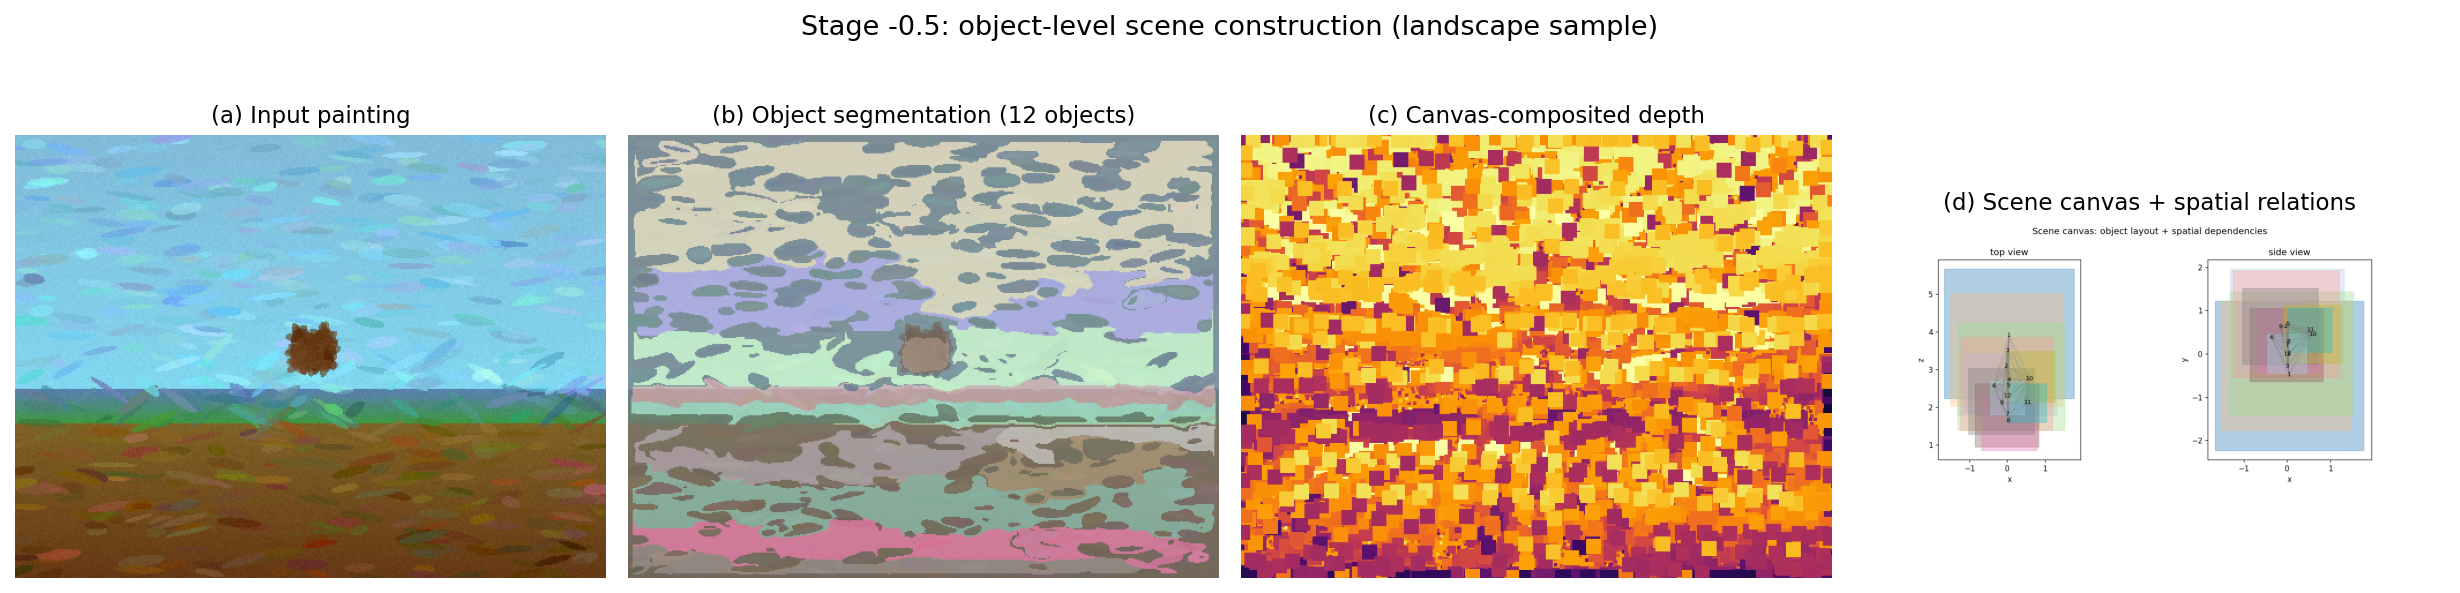
\includegraphics[width=0.98\linewidth]{figures/canvas_stage.png}
\caption{\textbf{Stage -0.5: object-level scene construction} (landscape
sample). (a)~Input painting. (b)~Depth-aware object segmentation: 12
instances (colour-tinted) with an objectness ranking; unassigned pixels
form the background set. (c)~The canvas-composited depth $D_c$ consumed by
the Stage-0 depth-warp control: a per-object splat z-buffer, so occlusion
boundaries are correct object silhouettes rather than raw depth edges.
(d)~The scene canvas: placed objects (top-down $x$--$z$ and side $x$--$y$
views) with their spatial-dependency edges; floating objects with
rests-on-ground relations were snapped onto the fitted ground plane.}
\label{fig:canvas}
\end{figure*}

% ---------------------------------------------------------------------
\subsection{Stage 0: Painting-conditioned video generation}
\label{sec:stage0}

We generate a flythrough $\{I_t\}_{t=1}^{N}$ along a camera trajectory
$\{T_t\}_{t=1}^{N}$ (orbit, dolly, pan, or spiral), with $T_1$ the painting's
viewpoint. The painting conditions the VDM through three 3D-stability
controls.

\paragraph{Depth-warp geometry control.}
At each frame $t$, we warp the canvas-composited depth $D_c$ (Stage -0.5;
the raw painting depth $D_p$ when the canvas is disabled) from $T_1$ to
$T_t$ by unprojecting, transforming, and re-projecting:
\begin{equation}
D_c^{(t)} = \Pi\!\left(T_t^{-1}\, T_1\, \Pi^{-1}(D_c)\right),
\end{equation}
where $\Pi$ denotes the camera projection. Because $D_c$ is z-buffered per
object, the control respects object occlusion boundaries: a foreground
object correctly hides the geometry behind it as the camera moves. The
warped depth $\{D_c^{(t)}\}_{t=1}^{N}$ is supplied to a depth ControlNet as
a per-frame geometry control. We blend the warped depth with the source
depth by a strength $\alpha \in [0,1]$:
\begin{equation}
\tilde{D}_c^{(t)} = \alpha\, D_c^{(t)} + (1-\alpha)\, D_c,
\end{equation}
so the control never drifts too far from the canvas layout. $\alpha$ is
the user-facing \texttt{depth\_warp\_control\_strength} knob.

\paragraph{Stroke-consistency attention.}
We lock the painting as the reference frame in the VDM's temporal attention
and add a stroke-mask attention bias $B \in \mathbb{R}^{N\times K\times K}$
(where $K$ is the number of tokens per frame) so that tokens belonging to the
same stroke segment $S_p$ attend preferentially to their counterparts in the
reference frame:
\begin{equation}
B_{t,i,j} = \!\begin{cases}
\!+1 & \text{if } S_p(i)\!=\!S_p(j)\!>\!0, \\
\!-0.25 & \text{if } S_p(i)\!\neq\!S_p(j),\, S_p(i),S_p(j)\!>\!0, \\
\;0 & \text{otherwise.}
\end{cases}
\end{equation}
This prevents brush strokes from drifting across frames.

\paragraph{Temporal-consistency guidance.}
During sampling we add a temporal-consistency guidance term with weight
$\beta$ that pulls each generated frame toward a temporally-smoothed
neighbour, reducing flicker.

% ---------------------------------------------------------------------
\subsection{Stage 1: Painting-anchored non-rigid alignment}
\label{sec:stage1}

We extend the non-rigid frame-to-model ICP
of~\cite{hoellein2026worldreconstruction}. The original method fixes frame
$j{=}0$ as the gauge fix and aligns each subsequent frame $k$ to the
accumulated canonical model via a per-frame SE(3) twist and a hash-grid local
deformation field, with energy
\begin{equation}
E = \mathcal{L}_\text{data} + \lambda_c\, \mathcal{L}_\text{color}
+ \lambda_r\, \mathcal{L}_\text{corr} + \lambda_t\, \mathcal{L}_\text{tv}.
\label{eq:icp}
\end{equation}
We make two painting-anchored modifications.

\paragraph{Painting-anchored canonical initialisation.}
Instead of fixing video frame $0$ as the canonical reference, we initialise
the canonical cloud from the painting's estimated geometry $\mathcal{P}_p$.
This is a stronger prior than any single generated frame because the painting
is the user-authored ground-truth appearance. We add a painting-anchor loss
that pulls the refined canonical cloud $\mathcal{P}_c$ toward $\mathcal{P}_p$:
\begin{equation}
\mathcal{L}_\text{anchor} = \frac{1}{|\mathcal{P}_c|}\sum_{x \in \mathcal{P}_c}
w(\mathrm{NN}(x))\, \|x - \mathrm{NN}(x)\|^2,
\end{equation}
where $\mathrm{NN}(x)$ is the nearest neighbour of $x$ in $\mathcal{P}_p$ and
$w$ is the painting confidence. The full Stage-1 energy becomes
$E + \lambda_a\, \mathcal{L}_\text{anchor}$.

\paragraph{Depth-warp per-point consistency.}
For each generated frame $k$ we compute a per-point consistency score $s_i
\in [0,1]$ by comparing each point's depth $z_i$ to the painting's depth
warped into frame $k$'s viewpoint, $D_p^{(k)}$:
\begin{equation}
s_i = \max\!\left(0,\; 1 - \frac{|z_i - D_p^{(k)}(u_i,v_i)|}
{\tau\, D_p^{(k)}(u_i,v_i)}\right),
\end{equation}
where $(u_i,v_i)$ is the point's pixel location and $\tau$ is a relative
tolerance. The score $s_i$ multiplies the point's residual in
$\mathcal{L}_\text{data}$, so points that drift beyond $\tau$ are
downweighted. This allows the scene to plausibly extend beyond the painting's
frustum (where $D_p^{(k)}$ is undefined and the score defaults to a small
constant) while suppressing drift within it.

% ---------------------------------------------------------------------
\subsection{Stage 3.2: Stroke-coherent, object-rigid 3D Gaussian Splatting}
\label{sec:stage3}

We initialise a 3D Gaussian Splatting scene $\mathcal{G}$
from the canvas $\mathcal{C}$ (the placed object Gaussians plus background)
when the object branch is enabled, and from the painting-initialised
canonical cloud $\mathcal{P}_c$ otherwise, and optimise it with the rendering
loss of~\cite{hoellein2026worldreconstruction} plus three painting-anchored
losses.

\paragraph{Stroke-coherence loss.}
We transfer the painting's stroke segmentation $S_p$ onto the 3D Gaussians by
projecting each Gaussian into the painting's viewpoint and reading the stroke
label. Let $\ell_g$ be the stroke label of Gaussian $g$ and $\phi_g$ its SH
DC colour. We penalise colour variance \emph{within} a stroke and reward
distance \emph{across} stroke boundaries:
\begin{align}
\mathcal{L}_\text{stroke} =\; & \lambda_\text{intra}\,
\frac{\sum_{(g,h)\in \mathcal{N}_{\ell_g}} \|\phi_g\!-\!\phi_h\|^2}
{|\mathcal{N}_{\ell_g}|} \nonumber\\
& +\, \lambda_\text{inter}\,
\overline{\big[m - \|\phi_g\!-\!\phi_h\|\big]_+}\,,
\end{align}
where $\mathcal{N}_{\ell_g}=\{(g,h)\!\in\!\mathcal{N}\!:\!\ell_g\!=\!\ell_h\!>\!0\}$
is the intra-stroke neighbour set, $\mathcal{N}$ the full Gaussian-neighbour
set, and $m$ an inter-stroke colour margin.

\paragraph{Painting-view reconstruction loss.}
The trained scene rendered from the painting's camera $T_1$ should reproduce
the input painting:
\begin{equation}
\mathcal{L}_\text{paint} = \|R(\mathcal{G}, T_1) - I_p\|_1 + \lambda_\text{lpips}\,
\mathrm{LPIPS}(R(\mathcal{G}, T_1), I_p).
\end{equation}

\paragraph{Object-rigid anchors and relation preservation.}
With the canvas enabled, scene optimisation must not tear the composed scene
apart: an object's Gaussians should move \emph{as a whole}, and the
dependency graph $\mathcal{R}$ should survive optimisation. We therefore
parameterise each object $o$'s motion by a learnable SE(3) delta
$(\Delta R_o, \Delta t_o)$ about its centroid --- a yaw for the vertical axis
plus a translation --- applied rigidly to all of $o$'s Gaussians, while
background Gaussians share a single delta; SH colours and opacities remain
per-Gaussian free parameters:
\begin{equation}
x_g' = c_o + \Delta R_o\,(x_g - c_o) + \Delta t_o, \quad g \in o.
\end{equation}
A \emph{relation-preservation loss} pins the support contacts of
$\mathcal{R}$: for every \emph{rests-on}$(a,b)$ (or rests-on-ground) edge
with initial contact gap $\gamma_0$, we penalise the drift of the current
gap $\gamma$ from its initial value,
\begin{equation}
\mathcal{L}_\text{rel} =
\frac{1}{|\mathcal{R}_\text{sup}|}
\sum_{(a,b)\in\mathcal{R}_\text{sup}}
\big|\,\gamma(a,b) - \gamma_0(a,b)\,\big|.
\end{equation}
Together the rigid anchors and $\mathcal{L}_\text{rel}$ let the optimiser
photometrically refine the scene --- nudging objects into place, adjusting
colours --- without objects interpenetrating, floating, or losing their
supports. The full Stage-3.2 loss is
$\mathcal{L}_\text{rend} + \lambda_s\, \mathcal{L}_\text{stroke} + \lambda_p\,
\mathcal{L}_\text{paint} + \lambda_r\, \mathcal{L}_\text{rel}$.
